%----------------------------------------------------------------------------------------
%    PACKAGES AND THEMES
%----------------------------------------------------------------------------------------
\documentclass[aspectratio=169,xcolor=dvipsnames]{beamer}
\makeatletter
\def\input@path{{../BeamerTemplate/theme/}}
\makeatother
\usetheme{CleanEasy}
\usepackage[utf8]{inputenc}
\usepackage{lmodern}
\usepackage[T1]{fontenc}
\usepackage{fix-cm}
\usepackage{amsmath}
\usepackage{mathtools}
\usepackage{listings}
\usepackage{xcolor}
\usepackage{hyperref}
\usepackage{graphicx}
\usepackage{booktabs}
\usepackage{tikz}
\usetikzlibrary{positioning, shapes, arrows, calc, decorations.pathreplacing, arrows.meta, backgrounds, patterns, overlay-beamer-styles}
\usepackage{etoolbox}

%----------------------------------------------------------------------------------------
%    LAYOUT CONFIGURATION
%----------------------------------------------------------------------------------------
\input{../BeamerTemplate/configs/configs}

%----------------------------------------------------------------------------------------
%    TITLE PAGE CONFIGURATION
%----------------------------------------------------------------------------------------
\title{Interview \& Competitive Programming Prep}
\subtitle{Targeted Practice to Master Patterns and Speed}
\author{Minseok Jeon}
\institute{DGIST}
\date{\today}

\begin{document}

\begin{frame}
  \titlepage
\end{frame}

\begin{frame}{Outline}
  \tableofcontents
\end{frame}

% Introduction
\section{Introduction}

\begin{frame}{Course Overview}
  \begin{block}{Goal}
    Master data structures and algorithms for technical interviews and competitive programming
  \end{block}

  \vspace{0.3cm}
  \textbf{Key Topics:}
  \begin{itemize}
    \item Common patterns for arrays, strings, stacks, queues
    \item Daily problem-solving routines
    \item Time complexity estimation techniques
    \item Pattern recognition and templates
    \item Mock interviews and reviews
    \item Progress tracking and metrics
  \end{itemize}
\end{frame}

\begin{frame}{Why This Preparation Matters}
  \begin{columns}
    \begin{column}{0.5\textwidth}
      \textbf{Technical Interviews:}
      \begin{itemize}
        \item FAANG companies emphasize DSA
        \item 45-60 minute coding interviews
        \item Communication is crucial
        \item Optimization expected
        \item Pattern recognition wins
      \end{itemize}
    \end{column}

    \begin{column}{0.5\textwidth}
      \textbf{Competitive Programming:}
      \begin{itemize}
        \item Speed + accuracy under time pressure
        \item Multiple problems in limited time
        \item Edge case handling
        \item Template mastery
        \item Algorithm optimization
      \end{itemize}
    \end{column}
  \end{columns}

  \vspace{0.3cm}
  \begin{alertblock}{Key Insight}
    Success requires deliberate practice with patterns, not just solving random problems
  \end{alertblock}
\end{frame}

% Arrays/Strings/Stacks/Queues Patterns
\section{Common Patterns}

\begin{frame}{Pattern Category Overview}
  \begin{table}
    \centering
    \small
    \begin{tabular}{lll}
      \hline
      \textbf{Data Structure} & \textbf{Common Patterns} & \textbf{Time Complexity} \\
      \hline
      Arrays/Strings & Two pointers, Sliding window & $O(n)$ \\
      Stacks & Monotonic stack, Parentheses & $O(n)$ \\
      Queues & BFS, Sliding window max & $O(n)$ \\
      Hash Tables & Frequency count, Anagrams & $O(n)$ \\
      \hline
    \end{tabular}
  \end{table}

  \vspace{0.3cm}
  \textbf{Learning Strategy:}
  \begin{enumerate}
    \item Recognize the pattern from problem description
    \item Apply the standard template
    \item Modify template for specific constraints
    \item Verify with test cases
  \end{enumerate}
\end{frame}

\subsection{Two Pointers Pattern}

\begin{frame}{Two Pointers: Concept}
  \begin{columns}
    \begin{column}{0.5\textwidth}
      \textbf{Pattern Description:}
      \begin{itemize}
        \item Use two indices moving through data
        \item Avoid nested loops ($O(n^2) \to O(n)$)
        \item Works on sorted or unsorted arrays
      \end{itemize}

      \vspace{0.3cm}
      \textbf{Variants:}
      \begin{itemize}
        \item Opposite direction (start/end)
        \item Same direction (fast/slow)
        \item Multiple arrays
      \end{itemize}
    \end{column}

    \begin{column}{0.5\textwidth}
      \textbf{Signal Words:}
      \begin{itemize}
        \item ``Pairs summing to...''
        \item ``Remove duplicates''
        \item ``Reverse in-place''
        \item ``Container/water problem''
        \item ``Palindrome check''
      \end{itemize}

      \vspace{0.3cm}
      \textbf{Complexity:}
      \begin{itemize}
        \item Time: $O(n)$ single pass
        \item Space: $O(1)$ in-place
      \end{itemize}
    \end{column}
  \end{columns}
\end{frame}

\begin{frame}[fragile]{Two Pointers: Template}
\begin{lstlisting}[language=Python, basicstyle=\small\ttfamily]
def two_pointers_template(arr):
    """Opposite direction pointers."""
    left, right = 0, len(arr) - 1

    while left < right:
        # Check condition
        if condition_met(arr[left], arr[right]):
            # Process and move both
            left += 1
            right -= 1
        elif need_larger_value:
            left += 1
        else:
            right -= 1

    return result
\end{lstlisting}

\textbf{Example: Two Sum (Sorted Array)}
\begin{itemize}
  \item Given sorted array, find indices where \texttt{arr[i] + arr[j] == target}
  \item If sum too small $\to$ move left pointer right
  \item If sum too large $\to$ move right pointer left
\end{itemize}
\end{frame}

\begin{frame}{Two Pointers: Visual Example}
  \begin{center}
    \textbf{Problem: Container with Most Water}

    \vspace{0.3cm}
    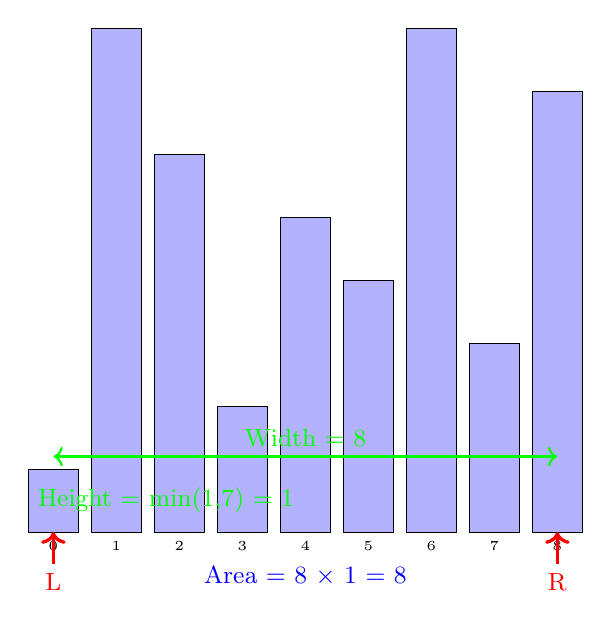
\begin{tikzpicture}[scale=0.8]
      % Height bars
      \foreach \x/\h in {0/1, 1/8, 2/6, 3/2, 4/5, 5/4, 6/8, 7/3, 8/7} {
        \draw[fill=blue!30] (\x, 0) rectangle (\x+0.8, \h);
        \node[below] at (\x+0.4, 0) {\tiny \x};
      }

      % Initial pointers
      \draw[->, very thick, red] (0.4, -0.5) -- (0.4, 0);
      \node[below, red] at (0.4, -0.5) {\small L};

      \draw[->, very thick, red] (8.4, -0.5) -- (8.4, 0);
      \node[below, red] at (8.4, -0.5) {\small R};

      % Area calculation
      \draw[<->, thick, green] (0.4, 1.2) -- (8.4, 1.2);
      \node[above, green, font=\small] at (4.4, 1.2) {Width = 8};
      \node[right, green, font=\small] at (0, 0.5) {Height = min(1,7) = 1};
      \node[above, blue, font=\small] at (4.4, -1) {Area = 8 $\times$ 1 = 8};
    \end{tikzpicture}
  \end{center}

  \vspace{0.2cm}
  \textbf{Strategy:}
  \begin{itemize}
    \item Start with widest container (left=0, right=n-1)
    \item Area = min(height[left], height[right]) $\times$ (right - left)
    \item Move pointer with smaller height inward
    \item Track maximum area
  \end{itemize}
\end{frame}

\subsection{Sliding Window Pattern}

\begin{frame}{Sliding Window: Concept}
  \begin{columns}
    \begin{column}{0.5\textwidth}
      \textbf{Pattern Description:}
      \begin{itemize}
        \item Maintain a window over data
        \item Expand/contract window dynamically
        \item Track window properties
        \item Avoid recomputing from scratch
      \end{itemize}

      \vspace{0.3cm}
      \textbf{Types:}
      \begin{itemize}
        \item \textbf{Fixed size}: Window size constant
        \item \textbf{Variable size}: Window grows/shrinks
      \end{itemize}
    \end{column}

    \begin{column}{0.5\textwidth}
      \textbf{Signal Words:}
      \begin{itemize}
        \item ``Contiguous subarray''
        \item ``Longest substring''
        \item ``Maximum/minimum in window''
        \item ``K consecutive elements''
      \end{itemize}

      \vspace{0.3cm}
      \textbf{Complexity:}
      \begin{itemize}
        \item Time: $O(n)$ (each element visited $\le$ 2 times)
        \item Space: $O(k)$ for window state
      \end{itemize}
    \end{column}
  \end{columns}
\end{frame}

\begin{frame}[fragile]{Sliding Window: Template}
\begin{lstlisting}[language=Python, basicstyle=\tiny\ttfamily]
def sliding_window_variable(s):
    """Variable size sliding window."""
    left = 0
    result = 0
    window = {}  # Track window state

    for right in range(len(s)):
        # Expand window: add s[right]
        window[s[right]] = window.get(s[right], 0) + 1

        # Contract window if condition violated
        while window_invalid(window):
            window[s[left]] -= 1
            if window[s[left]] == 0:
                del window[s[left]]
            left += 1

        # Update result with current window
        result = max(result, right - left + 1)

    return result

def sliding_window_fixed(arr, k):
    """Fixed size sliding window."""
    window_sum = sum(arr[:k])  # Initial window
    max_sum = window_sum

    for i in range(k, len(arr)):
        window_sum = window_sum - arr[i-k] + arr[i]  # Slide
        max_sum = max(max_sum, window_sum)

    return max_sum
\end{lstlisting}
\end{frame}

\begin{frame}{Sliding Window: Example}
  \textbf{Problem: Longest Substring Without Repeating Characters}

  \vspace{0.3cm}
  \begin{center}
    \texttt{s = "abcabcbb"}
  \end{center}

  \vspace{0.3cm}
  \begin{table}
    \centering
    \tiny
    \begin{tabular}{ccccc}
      \hline
      \textbf{Step} & \textbf{Window} & \textbf{Left} & \textbf{Right} & \textbf{Max Length} \\
      \hline
      1 & [a] & 0 & 0 & 1 \\
      2 & [a,b] & 0 & 1 & 2 \\
      3 & [a,b,c] & 0 & 2 & 3 \\
      4 & [a,b,c,a] $\to$ [b,c,a] & 1 & 3 & 3 \\
      5 & [b,c,a,b] $\to$ [c,a,b] & 2 & 4 & 3 \\
      6 & [c,a,b,c] $\to$ [a,b,c] & 3 & 5 & 3 \\
      \hline
    \end{tabular}
  \end{table}

  \vspace{0.3cm}
  \textbf{Answer: 3} (substring ``abc'')

  \vspace{0.2cm}
  \textbf{Key Idea:}
  \begin{itemize}
    \item Use hash map to track character positions
    \item When duplicate found, contract window from left
    \item Track maximum window size seen
  \end{itemize}
\end{frame}

\subsection{Stack Patterns}

\begin{frame}{Stack Patterns: Overview}
  \begin{columns}
    \begin{column}{0.5\textwidth}
      \textbf{Common Stack Patterns:}
      \begin{itemize}
        \item \textbf{Monotonic stack}: Next greater/smaller element
        \item \textbf{Parentheses matching}: Valid expressions
        \item \textbf{Expression evaluation}: Calculator, RPN
        \item \textbf{Backtracking}: DFS traversal
      \end{itemize}
    \end{column}

    \begin{column}{0.5\textwidth}
      \textbf{Signal Words:}
      \begin{itemize}
        \item ``Next greater element''
        \item ``Valid parentheses''
        \item ``Evaluate expression''
        \item ``Largest rectangle''
        \item ``Trapping rain water''
      \end{itemize}

      \vspace{0.3cm}
      \textbf{Why Stacks?}
      \begin{itemize}
        \item LIFO matches nested structures
        \item Efficient backtracking
        \item $O(1)$ push/pop operations
      \end{itemize}
    \end{column}
  \end{columns}
\end{frame}

\begin{frame}[fragile]{Monotonic Stack Pattern}
\begin{lstlisting}[language=Python, basicstyle=\tiny\ttfamily]
def next_greater_element(nums):
    """Find next greater element for each element."""
    n = len(nums)
    result = [-1] * n
    stack = []  # Store indices

    for i in range(n):
        # While current element is greater than stack top
        while stack and nums[i] > nums[stack[-1]]:
            idx = stack.pop()
            result[idx] = nums[i]
        stack.append(i)

    return result

# Example: nums = [2, 1, 2, 4, 3]
# Result: [4, 2, 4, -1, -1]
\end{lstlisting}

\vspace{0.2cm}
\textbf{Key Idea:}
\begin{itemize}
  \item Maintain stack in increasing/decreasing order
  \item Pop elements that violate monotonic property
  \item Each element pushed and popped once $\to$ $O(n)$
\end{itemize}
\end{frame}

\begin{frame}{Monotonic Stack: Visual Example}
  \textbf{Problem: Daily Temperatures}

  Given temperatures = [73, 74, 75, 71, 69, 72, 76, 73], find how many days until warmer temperature.

  \vspace{0.3cm}
  \begin{center}
    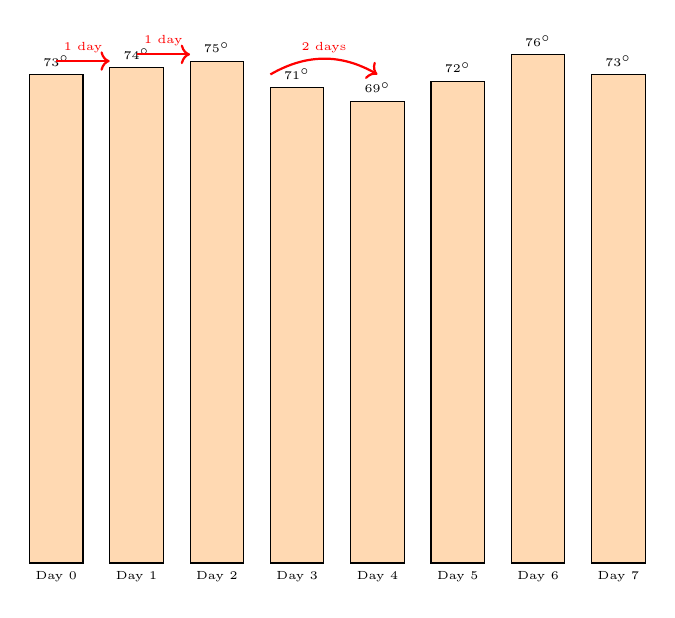
\begin{tikzpicture}[scale=0.85, every node/.style={scale=0.85}]
      % Temperature bars
      \foreach \x/\t in {0/73, 1/74, 2/75, 3/71, 4/69, 5/72, 6/76, 7/73} {
        \pgfmathsetmacro{\h}{\t/10}
        \draw[fill=orange!30] (\x*1.2, 0) rectangle (\x*1.2+0.8, \h);
        \node[below] at (\x*1.2+0.4, 0) {\tiny Day \x};
        \node[above] at (\x*1.2+0.4, \h) {\tiny \t$^\circ$};
      }

      % Arrows showing answers
      \draw[->, thick, red] (0.4, 7.5) -- (1.2, 7.5);
      \node[above, red, font=\tiny] at (0.8, 7.5) {1 day};

      \draw[->, thick, red] (1.6, 7.6) -- (2.4, 7.6);
      \node[above, red, font=\tiny] at (2.0, 7.6) {1 day};

      \draw[->, thick, red] (3.6, 7.3) to[bend left] (5.2, 7.3);
      \node[above, red, font=\tiny] at (4.4, 7.5) {2 days};
    \end{tikzpicture}
  \end{center}

  \vspace{0.2cm}
  \textbf{Answer: [1, 1, 4, 2, 1, 1, 0, 0]}

  \vspace{0.2cm}
  \textbf{Algorithm:}
  \begin{itemize}
    \item Use stack to store indices of temperatures
    \item For each day, pop all colder days and record distance
    \item Decreasing monotonic stack ensures $O(n)$ time
  \end{itemize}
\end{frame}

\begin{frame}[fragile]{Valid Parentheses Pattern}
\begin{lstlisting}[language=Python, basicstyle=\small\ttfamily]
def is_valid_parentheses(s):
    """Check if parentheses are balanced."""
    stack = []
    pairs = {'(': ')', '[': ']', '{': '}'}

    for char in s:
        if char in pairs:  # Opening bracket
            stack.append(char)
        else:  # Closing bracket
            if not stack or pairs[stack[-1]] != char:
                return False
            stack.pop()

    return len(stack) == 0

# Examples:
# "()" -> True
# "()[]{}" -> True
# "(]" -> False
# "([)]" -> False
# "{[]}" -> True
\end{lstlisting}
\end{frame}

\subsection{Queue Patterns}

\begin{frame}{Queue Patterns: Overview}
  \begin{columns}
    \begin{column}{0.5\textwidth}
      \textbf{Common Queue Patterns:}
      \begin{itemize}
        \item \textbf{BFS traversal}: Level-order, shortest path
        \item \textbf{Sliding window maximum}: Deque optimization
        \item \textbf{Level processing}: Binary tree levels
        \item \textbf{Multi-source BFS}: Multiple starting points
      \end{itemize}
    \end{column}

    \begin{column}{0.5\textwidth}
      \textbf{Signal Words:}
      \begin{itemize}
        \item ``Level order traversal''
        \item ``Shortest path''
        \item ``Minimum steps''
        \item ``Layer by layer''
        \item ``Sliding window maximum''
      \end{itemize}

      \vspace{0.3cm}
      \textbf{Why Queues?}
      \begin{itemize}
        \item FIFO ensures level-order processing
        \item Guarantees shortest path in unweighted graphs
        \item Natural for breadth-first exploration
      \end{itemize}
    \end{column}
  \end{columns}
\end{frame}

\begin{frame}[fragile]{BFS Template}
\begin{lstlisting}[language=Python, basicstyle=\tiny\ttfamily]
from collections import deque

def bfs_template(start):
    """Standard BFS traversal."""
    queue = deque([start])
    visited = {start}

    while queue:
        node = queue.popleft()

        # Process current node
        process(node)

        # Add neighbors
        for neighbor in get_neighbors(node):
            if neighbor not in visited:
                visited.add(neighbor)
                queue.append(neighbor)

    return result

def bfs_level_order(root):
    """BFS with level tracking."""
    if not root:
        return []

    queue = deque([root])
    result = []

    while queue:
        level_size = len(queue)
        level = []

        for _ in range(level_size):
            node = queue.popleft()
            level.append(node.val)

            if node.left:
                queue.append(node.left)
            if node.right:
                queue.append(node.right)

        result.append(level)

    return result
\end{lstlisting}
\end{frame}

\begin{frame}{BFS: Visual Example}
  \textbf{Binary Tree Level Order Traversal}

  \vspace{0.3cm}
  \begin{center}
    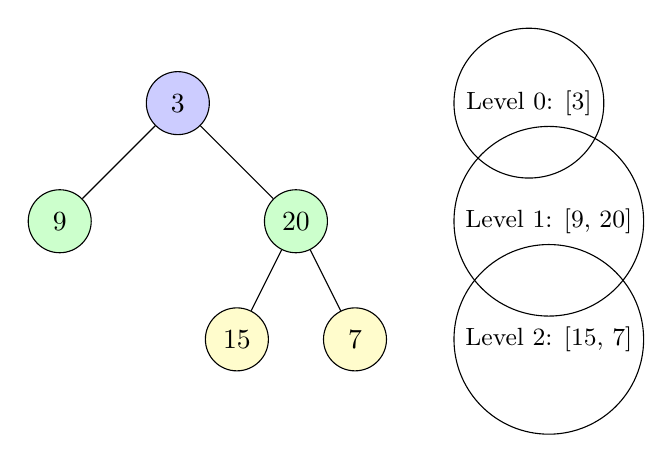
\begin{tikzpicture}[
      level distance=1.5cm,
      level 1/.style={sibling distance=3cm},
      level 2/.style={sibling distance=1.5cm},
      every node/.style={circle, draw, minimum size=0.8cm}
    ]
      \node[fill=blue!20] {3}
        child { node[fill=green!20] {9} }
        child { node[fill=green!20] {20}
          child { node[fill=yellow!20] {15} }
          child { node[fill=yellow!20] {7} }
        };

      % Level labels
      \node[right=3.5cm of {(0,0)}, font=\small] {Level 0: [3]};
      \node[right=3.5cm of {(0,-1.5)}, font=\small] {Level 1: [9, 20]};
      \node[right=3.5cm of {(0,-3)}, font=\small] {Level 2: [15, 7]};
    \end{tikzpicture}
  \end{center}

  \vspace{0.3cm}
  \textbf{Result: [[3], [9, 20], [15, 7]]}

  \vspace{0.2cm}
  \textbf{Key Points:}
  \begin{itemize}
    \item Process nodes level by level using queue
    \item Track level size to separate levels
    \item Each node visited exactly once $\to$ $O(n)$
  \end{itemize}
\end{frame}

% Daily Problem-Solving Routine
\section{Daily Problem-Solving Routine}

\begin{frame}{Building Consistent Practice Habits}
  \begin{block}{Core Principle}
    Consistency beats intensity. Daily practice builds pattern recognition and speed.
  \end{block}

  \vspace{0.3cm}
  \textbf{Recommended Schedule:}
  \begin{itemize}
    \item \textbf{Morning (30 min)}: 1 medium problem, fresh mind
    \item \textbf{Evening (20 min)}: Review solution, optimize, add to notes
    \item \textbf{Weekly (2 hours)}: Mock interview session
    \item \textbf{Monthly}: Review all problems, identify weak areas
  \end{itemize}

  \vspace{0.3cm}
  \textbf{Difficulty Progression:}
  \begin{itemize}
    \item Week 1-2: Easy problems (build confidence)
    \item Week 3-4: Mix 70\% easy, 30\% medium
    \item Week 5+: Mix 30\% easy, 60\% medium, 10\% hard
  \end{itemize}
\end{frame}

\begin{frame}{Topic Rotation Strategy}
  \begin{columns}
    \begin{column}{0.5\textwidth}
      \textbf{Weekly Rotation:}
      \begin{itemize}
        \item \textbf{Monday}: Arrays/Strings
        \item \textbf{Tuesday}: Stacks/Queues
        \item \textbf{Wednesday}: Trees/Graphs
        \item \textbf{Thursday}: Dynamic Programming
        \item \textbf{Friday}: Hash Tables/Heaps
        \item \textbf{Saturday}: Mixed review
        \item \textbf{Sunday}: Mock interview
      \end{itemize}
    \end{column}

    \begin{column}{0.5\textwidth}
      \textbf{Why Rotation?}
      \begin{itemize}
        \item Prevents burnout on single topic
        \item Builds breadth of knowledge
        \item Reinforces pattern recognition
        \item Mimics interview randomness
      \end{itemize}

      \vspace{0.3cm}
      \textbf{Time Boxing:}
      \begin{itemize}
        \item Easy: 15-20 min
        \item Medium: 25-35 min
        \item Hard: 40-50 min
        \item Stop and review solution if stuck
      \end{itemize}
    \end{column}
  \end{columns}
\end{frame}

\begin{frame}{Review Cycle: Spaced Repetition}
  \begin{center}
    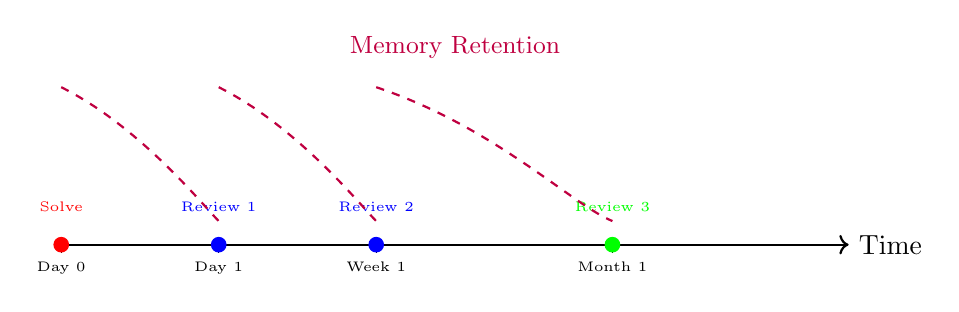
\begin{tikzpicture}[scale=1.0]
      % Timeline
      \draw[->, thick] (0, 0) -- (10, 0) node[right] {Time};

      % Day markers
      \foreach \x/\label in {0/Day 0, 2/Day 1, 4/Week 1, 7/Month 1} {
        \draw (\x, -0.1) -- (\x, 0.1);
        \node[below] at (\x, -0.1) {\tiny \label};
      }

      % Review points
      \node[circle, fill=red, inner sep=2pt] at (0, 0) {};
      \node[above, red, font=\tiny] at (0, 0.3) {Solve};

      \node[circle, fill=blue, inner sep=2pt] at (2, 0) {};
      \node[above, blue, font=\tiny] at (2, 0.3) {Review 1};

      \node[circle, fill=blue, inner sep=2pt] at (4, 0) {};
      \node[above, blue, font=\tiny] at (4, 0.3) {Review 2};

      \node[circle, fill=green, inner sep=2pt] at (7, 0) {};
      \node[above, green, font=\tiny] at (7, 0.3) {Review 3};

      % Memory curve
      \draw[dashed, thick, purple] (0, 2) .. controls (1, 1.5) and (1.8, 0.5) .. (2, 0.3);
      \draw[dashed, thick, purple] (2, 2) .. controls (3, 1.5) and (3.8, 0.5) .. (4, 0.3);
      \draw[dashed, thick, purple] (4, 2) .. controls (5.5, 1.5) and (6.5, 0.5) .. (7, 0.3);
      \node[purple, font=\small] at (5, 2.5) {Memory Retention};
    \end{tikzpicture}
  \end{center}

  \vspace{0.3cm}
  \textbf{Review Schedule:}
  \begin{itemize}
    \item \textbf{Day 1}: Re-solve without looking at notes (should be fresh)
    \item \textbf{Week 1}: Solve again, focus on optimization
    \item \textbf{Month 1}: Final review, add to template library if pattern
  \end{itemize}

  \vspace{0.2cm}
  \textbf{Goal}: Move problems from short-term to long-term memory
\end{frame}

\begin{frame}{Problem-Solving Workflow}
  \begin{enumerate}
    \item \textbf{Read \& Understand} (2-3 min)
    \begin{itemize}
      \item Read problem carefully, underline key constraints
      \item Ask clarifying questions (inputs, outputs, edge cases)
      \item Identify problem type/pattern
    \end{itemize}

    \vspace{0.2cm}
    \item \textbf{Plan Approach} (3-5 min)
    \begin{itemize}
      \item Discuss brute force solution first
      \item Identify optimizations (data structure, algorithm)
      \item Estimate time/space complexity
    \end{itemize}

    \vspace{0.2cm}
    \item \textbf{Code Solution} (15-20 min)
    \begin{itemize}
      \item Write clean, readable code
      \item Use meaningful variable names
      \item Add comments for complex logic
    \end{itemize}

    \vspace{0.2cm}
    \item \textbf{Test \& Debug} (5-7 min)
    \begin{itemize}
      \item Test with example cases
      \item Check edge cases (empty, single element, large input)
      \item Fix bugs systematically
    \end{itemize}

    \vspace{0.2cm}
    \item \textbf{Optimize \& Discuss} (3-5 min)
    \begin{itemize}
      \item Discuss alternative approaches
      \item Analyze trade-offs
      \item Consider follow-up questions
    \end{itemize}
  \end{enumerate}
\end{frame}

% Time Complexity Estimation
\section{Time Complexity Estimation}

\begin{frame}{Big-O Notation: Quick Reference}
  \begin{table}
    \centering
    \small
    \begin{tabular}{lll}
      \hline
      \textbf{Notation} & \textbf{Name} & \textbf{Example} \\
      \hline
      $O(1)$ & Constant & Hash table lookup \\
      $O(\log n)$ & Logarithmic & Binary search \\
      $O(n)$ & Linear & Single array pass \\
      $O(n \log n)$ & Linearithmic & Merge sort, heap operations \\
      $O(n^2)$ & Quadratic & Nested loops \\
      $O(n^3)$ & Cubic & Triple nested loops \\
      $O(2^n)$ & Exponential & Recursive backtracking \\
      $O(n!)$ & Factorial & All permutations \\
      \hline
    \end{tabular}
  \end{table}

  \vspace{0.3cm}
  \begin{alertblock}{Golden Rule}
    If unsure, count nested loops and recursion depth. Each nesting level typically multiplies complexity.
  \end{alertblock}
\end{frame}

\begin{frame}{Input Size Guidelines}
  \begin{table}
    \centering
    \begin{tabular}{cc}
      \hline
      \textbf{Input Size $n$} & \textbf{Maximum Acceptable Complexity} \\
      \hline
      $n \le 10$ & $O(n!)$, $O(2^n)$ \\
      $n \le 20$ & $O(2^n)$ \\
      $n \le 100$ & $O(n^3)$ \\
      $n \le 1,000$ & $O(n^2)$ \\
      $n \le 10,000$ & $O(n^2)$ with small constant \\
      $n \le 100,000$ & $O(n \log n)$ \\
      $n \le 1,000,000$ & $O(n)$ or $O(n \log n)$ \\
      $n \le 10,000,000$ & $O(n)$ \\
      \hline
    \end{tabular}
  \end{table}

  \vspace{0.3cm}
  \textbf{Rule of Thumb:}
  \begin{itemize}
    \item Modern computers: $\sim 10^8$ to $10^9$ operations per second
    \item Time limit typically 1-2 seconds
    \item Estimate: $n \times \text{complexity factor} < 10^8$
  \end{itemize}
\end{frame}

\begin{frame}{Complexity Analysis Examples}
  \begin{columns}
    \begin{column}{0.5\textwidth}
      \textbf{Example 1: Nested Loops}
      \begin{align*}
        &\text{for } i \text{ in range}(n): \\
        &\quad \text{for } j \text{ in range}(n): \\
        &\quad\quad \text{// } O(1) \text{ work}
      \end{align*}
      \textbf{Analysis:} $O(n \times n) = O(n^2)$

      \vspace{0.3cm}
      \textbf{Example 2: Divide and Conquer}
      \begin{align*}
        T(n) &= 2T(n/2) + O(n)
      \end{align*}
      \textbf{Analysis:} $O(n \log n)$ (Merge Sort)
    \end{column}

    \begin{column}{0.5\textwidth}
      \textbf{Example 3: Binary Search Tree}
      \begin{align*}
        &\text{while } \text{node} \ne \text{null}: \\
        &\quad \text{node} = \text{node.left or right}
      \end{align*}
      \textbf{Analysis:} $O(\log n)$ balanced, $O(n)$ worst

      \vspace{0.3cm}
      \textbf{Example 4: Sliding Window}
      \begin{align*}
        &\text{for } \text{right} \text{ in range}(n): \\
        &\quad \text{while } \text{invalid}: \\
        &\quad\quad \text{left} += 1
      \end{align*}
      \textbf{Analysis:} $O(n)$ (each element visited $\le$ 2 times)
    \end{column}
  \end{columns}
\end{frame}

\begin{frame}{Space-Time Tradeoffs}
  \begin{columns}
    \begin{column}{0.5\textwidth}
      \textbf{When to Use Extra Space:}
      \begin{itemize}
        \item Hash maps for $O(1)$ lookup
        \item Memoization in DP
        \item Caching intermediate results
        \item Preprocessing for multiple queries
      \end{itemize}

      \vspace{0.3cm}
      \textbf{Example: Two Sum}
      \begin{itemize}
        \item Brute force: $O(n^2)$ time, $O(1)$ space
        \item Hash map: $O(n)$ time, $O(n)$ space
      \end{itemize}
    \end{column}

    \begin{column}{0.5\textwidth}
      \textbf{When to Save Space:}
      \begin{itemize}
        \item Memory-constrained systems
        \item Large datasets
        \item In-place modifications allowed
        \item Space complexity matters
      \end{itemize}

      \vspace{0.3cm}
      \textbf{Example: Reverse Array}
      \begin{itemize}
        \item Extra array: $O(n)$ space
        \item Two pointers in-place: $O(1)$ space
      \end{itemize}
    \end{column}
  \end{columns}

  \vspace{0.3cm}
  \begin{block}{Interview Tip}
    Always discuss both time and space complexity. Mention trade-offs explicitly.
  \end{block}
\end{frame}

% Pattern Recognition and Templates
\section{Pattern Recognition}

\begin{frame}{Common Problem Categories}
  \begin{table}
    \centering
    \tiny
    \begin{tabular}{lll}
      \hline
      \textbf{Category} & \textbf{Signal Words} & \textbf{Approach} \\
      \hline
      Sliding Window & Contiguous subarray, substring & Two pointers, hash map \\
      Two Pointers & Sorted array, pairs, palindrome & Opposite or same direction \\
      Backtracking & All combinations, permutations & Recursive DFS with pruning \\
      Dynamic Programming & Optimal, maximum/minimum & Memoization or tabulation \\
      Graph Traversal & Connected components, paths & DFS for paths, BFS for shortest \\
      Binary Search & Sorted, find target/range & Divide search space \\
      Greedy & Locally optimal choices & Sort + greedy selection \\
      Divide \& Conquer & Break into subproblems & Merge sort, quick sort pattern \\
      \hline
    \end{tabular}
  \end{table}

  \vspace{0.3cm}
  \textbf{Pattern Recognition Strategy:}
  \begin{enumerate}
    \item Read problem, identify keywords
    \item Check constraints (sorted? tree? graph?)
    \item Recall similar problems solved before
    \item Apply matching template
  \end{enumerate}
\end{frame}

\begin{frame}[fragile]{Template Library: Binary Search}
\begin{lstlisting}[language=Python, basicstyle=\tiny\ttfamily]
def binary_search_exact(arr, target):
    """Find exact target."""
    left, right = 0, len(arr) - 1
    while left <= right:
        mid = left + (right - left) // 2
        if arr[mid] == target:
            return mid
        elif arr[mid] < target:
            left = mid + 1
        else:
            right = mid - 1
    return -1

def binary_search_left_bound(arr, target):
    """Find leftmost occurrence."""
    left, right = 0, len(arr)
    while left < right:
        mid = left + (right - left) // 2
        if arr[mid] < target:
            left = mid + 1
        else:
            right = mid
    return left

def binary_search_on_answer(check, low, high):
    """Binary search on answer space."""
    while low < high:
        mid = low + (high - low) // 2
        if check(mid):
            high = mid
        else:
            low = mid + 1
    return low
\end{lstlisting}
\end{frame}

\begin{frame}[fragile]{Template Library: Backtracking}
\begin{lstlisting}[language=Python, basicstyle=\tiny\ttfamily]
def backtrack_template(nums):
    """Generate all combinations/permutations."""
    result = []

    def backtrack(path, start):
        # Base case: path complete
        if is_complete(path):
            result.append(path[:])  # Copy current path
            return

        # Recursive case: try all choices
        for i in range(start, len(nums)):
            # Choose
            path.append(nums[i])

            # Explore
            backtrack(path, i + 1)  # i+1 for combinations, 0 for permutations

            # Unchoose (backtrack)
            path.pop()

    backtrack([], 0)
    return result

# Pruning optimization:
def backtrack_with_pruning(path, start):
    if not is_valid(path):  # Prune invalid paths early
        return
    # ... rest of backtracking logic
\end{lstlisting}
\end{frame}

\begin{frame}{Similar Problem Mapping}
  \textbf{Recognizing Problem Variations:}

  \vspace{0.3cm}
  \begin{table}
    \centering
    \tiny
    \begin{tabular}{ll}
      \hline
      \textbf{New Problem} & \textbf{Maps To} \\
      \hline
      Coin Change & Unbounded Knapsack DP \\
      House Robber & Linear DP with non-adjacent constraint \\
      Longest Increasing Subsequence & DP or Binary Search \\
      Edit Distance & 2D DP (Levenshtein distance) \\
      Word Break & DP with string matching \\
      Maximum Subarray & Kadane's algorithm \\
      Trapping Rain Water & Two pointers or monotonic stack \\
      Merge Intervals & Sorting + greedy \\
      Number of Islands & DFS/BFS on grid \\
      Clone Graph & DFS/BFS with hash map \\
      \hline
    \end{tabular}
  \end{table}

  \vspace{0.3cm}
  \textbf{Strategy:} Maintain a mental library of classic problems. New problems are often variations.
\end{frame}

% Mock Interviews and Reviews
\section{Mock Interviews}

\begin{frame}{Mock Interview Structure}
  \textbf{Simulating Real Interview Conditions (45-60 min):}

  \vspace{0.3cm}
  \begin{enumerate}
    \item \textbf{Introduction} (2-3 min)
    \begin{itemize}
      \item Brief self-introduction
      \item Interviewer explains format
    \end{itemize}

    \vspace{0.2cm}
    \item \textbf{Problem Presentation} (2-3 min)
    \begin{itemize}
      \item Read problem carefully
      \item Ask clarifying questions
      \item Confirm understanding
    \end{itemize}

    \vspace{0.2cm}
    \item \textbf{Discussion} (5-10 min)
    \begin{itemize}
      \item Explain brute force approach
      \item Discuss optimizations
      \item Agree on approach with interviewer
    \end{itemize}

    \vspace{0.2cm}
    \item \textbf{Coding} (20-25 min)
    \begin{itemize}
      \item Write clean, commented code
      \item Think aloud while coding
      \item Handle edge cases
    \end{itemize}

    \vspace{0.2cm}
    \item \textbf{Testing} (5-10 min)
    \begin{itemize}
      \item Walk through test cases
      \item Identify and fix bugs
    \end{itemize}

    \vspace{0.2cm}
    \item \textbf{Follow-up} (5 min)
    \begin{itemize}
      \item Discuss optimizations
      \item Answer follow-up questions
    \end{itemize}
  \end{enumerate}
\end{frame}

\begin{frame}{Communication Best Practices}
  \begin{columns}
    \begin{column}{0.5\textwidth}
      \textbf{Do's:}
      \begin{itemize}
        \item Think aloud consistently
        \item Ask clarifying questions
        \item Explain your reasoning
        \item Discuss trade-offs
        \item Admit when stuck, ask for hints
        \item Be open to feedback
        \item Stay calm and positive
      \end{itemize}

      \vspace{0.3cm}
      \textbf{Example Phrases:}
      \begin{itemize}
        \item ``I'm thinking of using a hash map because...''
        \item ``The time complexity would be $O(n)$ since...''
        \item ``Let me trace through an example...''
        \item ``Could I get a hint on...?''
      \end{itemize}
    \end{column}

    \begin{column}{0.5\textwidth}
      \textbf{Don'ts:}
      \begin{itemize}
        \item Code in silence
        \item Jump to coding without discussion
        \item Ignore interviewer's hints
        \item Get defensive about mistakes
        \item Give up when stuck
        \item Skip testing
        \item Ignore edge cases
      \end{itemize}

      \vspace{0.3cm}
      \textbf{Red Flags:}
      \begin{itemize}
        \item Not asking questions
        \item Poor variable naming
        \item Skipping complexity analysis
        \item Not testing solution
        \item Messy, unreadable code
      \end{itemize}
    \end{column}
  \end{columns}
\end{frame}

\begin{frame}{Mock Interview Platforms}
  \begin{columns}
    \begin{column}{0.5\textwidth}
      \textbf{Free Platforms:}
      \begin{itemize}
        \item \textbf{LeetCode Mock Interviews}: Timed problems with evaluation
        \item \textbf{Pramp}: Peer-to-peer mock interviews
        \item \textbf{CodeSignal}: Assessment practice
        \item \textbf{HackerRank}: Interview prep kits
      \end{itemize}

      \vspace{0.3cm}
      \textbf{Paid Platforms:}
      \begin{itemize}
        \item \textbf{interviewing.io}: Anonymous interviews with engineers
        \item \textbf{Exponent}: Mock interviews with feedback
        \item \textbf{Brilliant.org}: Interactive problem solving
      \end{itemize}
    \end{column}

    \begin{column}{0.5\textwidth}
      \textbf{Practice Partners:}
      \begin{itemize}
        \item Study groups
        \item Friends preparing for interviews
        \item Online communities (Reddit, Discord)
        \item University career services
      \end{itemize}

      \vspace{0.3cm}
      \textbf{Recording \& Review:}
      \begin{itemize}
        \item Record your sessions (with permission)
        \item Review recordings later
        \item Identify communication gaps
        \item Track improvement over time
      \end{itemize}
    \end{column}
  \end{columns}
\end{frame}

\begin{frame}{Post-Mortem Analysis}
  \textbf{After Each Mock Interview:}

  \vspace{0.3cm}
  \begin{enumerate}
    \item \textbf{What Went Well:}
    \begin{itemize}
      \item Clear communication
      \item Correct solution found
      \item Good time management
      \item Handled edge cases
    \end{itemize}

    \vspace{0.2cm}
    \item \textbf{What to Improve:}
    \begin{itemize}
      \item Missed initial edge case (empty array)
      \item Took too long to code (30 min instead of 20 min)
      \item Didn't discuss space complexity
      \item Nervous, spoke too fast
    \end{itemize}

    \vspace{0.2cm}
    \item \textbf{Alternative Approaches:}
    \begin{itemize}
      \item Could have used DP instead of recursion
      \item Hash map would have been simpler
      \item Greedy approach also works here
    \end{itemize}

    \vspace{0.2cm}
    \item \textbf{Action Items:}
    \begin{itemize}
      \item Practice similar problems (10 more DP problems)
      \item Review edge case checklist before coding
      \item Work on speaking pace and clarity
    \end{itemize}
  \end{enumerate}
\end{frame}

% Tracking Progress and Metrics
\section{Progress Tracking}

\begin{frame}{Problem Log Template}
  \textbf{Spreadsheet/Notion Tracking:}

  \vspace{0.3cm}
  \begin{table}
    \centering
    \tiny
    \begin{tabular}{llllll}
      \hline
      \textbf{Date} & \textbf{Problem} & \textbf{Difficulty} & \textbf{Time} & \textbf{Status} & \textbf{Notes} \\
      \hline
      11/01 & Two Sum & Easy & 15 min & \checkmark & Hash map approach \\
      11/01 & Valid Parentheses & Easy & 20 min & \checkmark & Stack, clean solution \\
      11/02 & Longest Substring & Medium & 45 min & \checkmark & Struggled with sliding window \\
      11/02 & Merge Intervals & Medium & 35 min & \checkmark & Sorting + greedy \\
      11/03 & Binary Tree Level Order & Medium & 30 min & \checkmark & BFS with queue \\
      11/03 & Coin Change & Medium & 60 min & $\times$ & Need to review DP \\
      \hline
    \end{tabular}
  \end{table}

  \vspace{0.3cm}
  \textbf{Key Metrics to Track:}
  \begin{itemize}
    \item Solve time per difficulty
    \item Success rate per topic
    \item Common mistakes
    \item Review schedule adherence
  \end{itemize}
\end{frame}

\begin{frame}{Topic Coverage Checklist}
  \begin{columns}
    \begin{column}{0.5\textwidth}
      \textbf{Data Structures:}
      \begin{itemize}
        \item[\checkmark] Arrays (85\% proficiency)
        \item[\checkmark] Strings (80\% proficiency)
        \item[\checkmark] Stacks (90\% proficiency)
        \item[\checkmark] Queues (85\% proficiency)
        \item[\checkmark] Hash Tables (80\% proficiency)
        \item[$\triangle$] Trees (65\% proficiency)
        \item[$\triangle$] Graphs (60\% proficiency)
        \item[$\times$] Heaps (45\% proficiency)
        \item[$\times$] Tries (40\% proficiency)
      \end{itemize}
    \end{column}

    \begin{column}{0.5\textwidth}
      \textbf{Algorithms:}
      \begin{itemize}
        \item[\checkmark] Two Pointers (85\%)
        \item[\checkmark] Sliding Window (80\%)
        \item[\checkmark] Binary Search (85\%)
        \item[$\triangle$] Backtracking (60\%)
        \item[$\triangle$] Dynamic Programming (55\%)
        \item[$\times$] Graph Algorithms (50\%)
        \item[\checkmark] Sorting (90\%)
        \item[$\triangle$] Greedy (65\%)
      \end{itemize}

      \vspace{0.3cm}
      \textbf{Legend:}
      \begin{itemize}
        \item[\checkmark] $\ge 80\%$: Strong
        \item[$\triangle$] 50-79\%: Needs practice
        \item[$\times$] $< 50\%$: Priority focus
      \end{itemize}
    \end{column}
  \end{columns}
\end{frame}

\begin{frame}{Speed Metrics and Goals}
  \begin{table}
    \centering
    \begin{tabular}{lccc}
      \hline
      \textbf{Difficulty} & \textbf{Target Time} & \textbf{Current Avg} & \textbf{Status} \\
      \hline
      Easy & 15-20 min & 18 min & \checkmark On track \\
      Medium & 25-35 min & 40 min & $\triangle$ Need improvement \\
      Hard & 40-50 min & 65 min & $\times$ Priority \\
      \hline
    \end{tabular}
  \end{table}

  \vspace{0.3cm}
  \textbf{Speed Improvement Strategies:}
  \begin{itemize}
    \item Focus on pattern recognition (reduce planning time)
    \item Master templates (reduce coding time)
    \item Practice typing speed and shortcuts
    \item Time-box practice sessions
    \item Review fast solutions from top submissions
  \end{itemize}

  \vspace{0.3cm}
  \begin{block}{Goal}
    Reduce medium problem time to 30 min within 2 months through daily practice
  \end{block}
\end{frame}

\begin{frame}{Identifying Weak Areas}
  \textbf{Analysis Methods:}

  \vspace{0.3cm}
  \begin{enumerate}
    \item \textbf{Problem Log Analysis}
    \begin{itemize}
      \item Filter by unsolved or struggled problems
      \item Group by topic/pattern
      \item Identify recurring difficulties
    \end{itemize}

    \vspace{0.2cm}
    \item \textbf{Time Analysis}
    \begin{itemize}
      \item Which topics take longest?
      \item Where do you get stuck? (planning, coding, debugging)
      \item Compare to target times
    \end{itemize}

    \vspace{0.2cm}
    \item \textbf{Success Rate by Topic}
    \begin{itemize}
      \item \% solved on first try
      \item \% requiring hint/solution lookup
      \item \% passing all test cases
    \end{itemize}

    \vspace{0.2cm}
    \item \textbf{Mock Interview Feedback}
    \begin{itemize}
      \item Interviewer notes
      \item Communication issues
      \item Technical gaps
    \end{itemize}
  \end{enumerate}
\end{frame}

\begin{frame}{Contest Participation}
  \begin{columns}
    \begin{column}{0.5\textwidth}
      \textbf{Weekly Contests:}
      \begin{itemize}
        \item \textbf{LeetCode Weekly/Biweekly}: Saturday/Sunday
        \item \textbf{Codeforces}: Multiple times per week
        \item \textbf{AtCoder Beginner Contest}: Weekly
        \item \textbf{CodeChef}: Long/short contests
      \end{itemize}

      \vspace{0.3cm}
      \textbf{Benefits:}
      \begin{itemize}
        \item Time pressure practice
        \item Ranking/percentile tracking
        \item Exposure to new problems
        \item Community solutions
      \end{itemize}
    \end{column}

    \begin{column}{0.5\textwidth}
      \textbf{Contest Strategy:}
      \begin{itemize}
        \item Read all problems first (5 min)
        \item Solve easiest problems first
        \item Submit early and often
        \item Don't get stuck on one problem
        \item Review solutions after contest
      \end{itemize}

      \vspace{0.3cm}
      \textbf{Rating Goals:}
      \begin{itemize}
        \item LeetCode: Target 1800+ (top 10\%)
        \item Codeforces: Target Expert (1600+)
        \item Track rating trends monthly
      \end{itemize}
    \end{column}
  \end{columns}
\end{frame}

% Summary
\section{Summary}

\begin{frame}{Key Takeaways}
  \begin{enumerate}
    \item \textbf{Master Common Patterns}
    \begin{itemize}
      \item Two pointers, sliding window, monotonic stack, BFS
      \item Templates save time and reduce errors
      \item Pattern recognition is the key to speed
    \end{itemize}

    \vspace{0.2cm}
    \item \textbf{Consistent Daily Practice}
    \begin{itemize}
      \item 1-3 problems daily with topic rotation
      \item Spaced repetition for long-term retention
      \item Time-boxed sessions to build speed
    \end{itemize}

    \vspace{0.2cm}
    \item \textbf{Complexity Analysis}
    \begin{itemize}
      \item Estimate before coding (saves time)
      \item Know input size $\to$ complexity mapping
      \item Discuss time/space trade-offs
    \end{itemize}

    \vspace{0.2cm}
    \item \textbf{Communication Matters}
    \begin{itemize}
      \item Think aloud in interviews
      \item Ask clarifying questions
      \item Explain approach before coding
    \end{itemize}

    \vspace{0.2cm}
    \item \textbf{Track and Optimize}
    \begin{itemize}
      \item Log every problem solved
      \item Identify weak areas systematically
      \item Participate in contests for benchmarking
    \end{itemize}
  \end{enumerate}
\end{frame}

\begin{frame}{12-Week Study Plan}
  \textbf{Structured Preparation Timeline:}

  \vspace{0.3cm}
  \begin{itemize}
    \item \textbf{Weeks 1-2: Foundations}
    \begin{itemize}
      \item Easy problems only (arrays, strings, stacks, queues)
      \item Build confidence and basic pattern recognition
      \item Target: 40-50 easy problems
    \end{itemize}

    \vspace{0.2cm}
    \item \textbf{Weeks 3-4: Expand Patterns}
    \begin{itemize}
      \item Mix 60\% easy, 40\% medium
      \item Trees, graphs, hash tables
      \item Target: 30 easy + 20 medium
    \end{itemize}

    \vspace{0.2cm}
    \item \textbf{Weeks 5-8: Core Medium Problems}
    \begin{itemize}
      \item Mix 30\% easy, 60\% medium, 10\% hard
      \item Focus on DP, backtracking, advanced patterns
      \item Weekly mock interviews
      \item Target: 15 easy + 40 medium + 5 hard
    \end{itemize}

    \vspace{0.2cm}
    \item \textbf{Weeks 9-12: Interview Ready}
    \begin{itemize}
      \item Mix 20\% easy, 60\% medium, 20\% hard
      \item Company-specific problem lists
      \item 2x mock interviews per week
      \item Target: 10 easy + 35 medium + 15 hard
    \end{itemize}
  \end{itemize}
\end{frame}

\begin{frame}{Resources and References}
  \begin{columns}
    \begin{column}{0.5\textwidth}
      \textbf{Problem Platforms:}
      \begin{itemize}
        \item LeetCode (most popular)
        \item HackerRank
        \item Codeforces
        \item AtCoder
        \item CodeChef
      \end{itemize}

      \vspace{0.3cm}
      \textbf{Books:}
      \begin{itemize}
        \item ``Cracking the Coding Interview'' (Gayle Laakmann McDowell)
        \item ``Elements of Programming Interviews''
        \item ``Competitive Programming'' (Halim \& Halim)
      \end{itemize}
    \end{column}

    \begin{column}{0.5\textwidth}
      \textbf{Online Resources:}
      \begin{itemize}
        \item NeetCode (pattern roadmap)
        \item AlgoExpert (curated problems)
        \item Blind 75 (essential problems)
        \item Grind 75 (study plan)
      \end{itemize}

      \vspace{0.3cm}
      \textbf{Communities:}
      \begin{itemize}
        \item r/leetcode
        \item LeetCode Discuss
        \item Codeforces Blogs
        \item Discord servers
      \end{itemize}
    \end{column}
  \end{columns}
\end{frame}

\begin{frame}{Final Advice}
  \begin{block}{Remember}
    Interview preparation is a marathon, not a sprint. Consistent practice beats cramming.
  \end{block}

  \vspace{0.3cm}
  \textbf{Mental Preparation:}
  \begin{itemize}
    \item Don't compare yourself to others (focus on your growth)
    \item It's okay to struggle with problems
    \item Learn from mistakes (they're valuable)
    \item Take breaks to avoid burnout
    \item Celebrate small wins (solved a hard problem!)
  \end{itemize}

  \vspace{0.3cm}
  \textbf{During the Interview:}
  \begin{itemize}
    \item Stay calm and think clearly
    \item Communication is 50\% of success
    \item It's okay to ask for hints
    \item Show your problem-solving process
    \item Be enthusiastic and positive
  \end{itemize}

  \vspace{0.3cm}
  \begin{alertblock}{You've Got This!}
    With consistent practice and pattern mastery, you will succeed!
  \end{alertblock}
\end{frame}

\begin{frame}
  \begin{center}
    {\Huge Thank You!}

    \vspace{1cm}
    {\Large Questions?}

    \vspace{1cm}
    \textit{``The only way to learn to program is by writing programs.'' -- Dennis Ritchie}

    \vspace{0.5cm}
    \small Apply this wisdom to interview prep: \\
    The only way to get better is by solving problems daily!

    \vspace{1cm}
    \textbf{Good luck with your interviews!}
  \end{center}
\end{frame}

\end{document}
